\documentclass[12pt]{article}

% Packages
\usepackage{tikz}
\usepackage[utf8]{inputenc}
\usepackage{graphicx}
\usepackage{enumerate}
\usepackage{tabularx}
\usepackage{longtable}
\usepackage{booktabs}
\usepackage{caption}
\usepackage{placeins}
\usepackage{float}
\usepackage{multirow}
\usepackage{graphicx}
\graphicspath{ {images/} }

\title{
ClinicFlow
\\\vspace{10mm}
\large \textbf{User Manual}
\vspace{40mm}
}
\author{ Maxim Vasiliev \#400043983\\
Susie Yu \#000955758\\
Karl Knopf \#001437217\\
Weilin Hu \#001150873\\
Yunfeng Li \#001335650
}
\date{March 3 2017}

\setlength\parindent{0pt}
\begin{document}
\pagenumbering{gobble}
\maketitle
\newpage
\tableofcontents
\listoffigures
\newpage
\pagenumbering{arabic}


\section{Introduction}

\subsection{What is ClinicFlow?}
ClinicFlow is a tool which allows clinics to: keep a record of patient activity data, generate statistics on past data, and simulate clinic environments to predict future performance.

\subsection{Objective of User Manual}
This manual provides an overview and guide for the core functionalities included in this product. If you have not yet created an account, please refer to section 4.
\medbreak

For all other inqueries, please refer to section 6. Tourbleshoooting. If this guide does not answer your questions, feel free to contact us: Section 6.2

\subsection{Background}
This tool was first developed for use at the Joseph Brant Hospital pre-operative clinic. Its functionality has since been expanded to allow changing of clinic properties, including staff, procedures, and additional constraints.

\subsection{Roadmap}
We hope to allow this product to be implemented in any clinic environment. To do this, we have taken steps to abstract away the specific clinic we are dealing with, instead opting for a variable clinic model which can be adapted to the specific clinic using this product.

\section{Legal / Copyright Info}
ClincFlow is owned and managed by the ClinicFlow team of McMaster University (See 6.2: Contact Us). The source code is available on github, and this product is licensed under GPLv3. The full text of which is available at:
\medbreak
https://www.gnu.org/licenses/gpl-3.0.en.html

\section{System Requirements}
ClinicFlow is a web application. It requires an operating system and browser supporting:
\newline
- HTML5
\medbreak
- CSS3
\medbreak
- Javascript
\medbreak

Compatible browsers include:
\medbreak
- Microsoft Internet Explorer 10+
\medbreak
- Microsoft Edge
\medbreak
- Google Chrome
\medbreak
- Mozilla Firefox
\medbreak
- Safari

\section{Account}
When first accessing the application, the login screen is presented. From here one can either enter an existing an account, or create a new one.

\subsection{Login}
The login screen consists of a Username and Password field. Both are required to login and use the application.
\medbreak

If you do not have an account, please refer to the Registration section (4.2)
\medbreak

To Sign In:
\medbreak
1. Enter your username into the "Username" box
\medbreak
2. Enter your password into the "Password" box
\medbreak
3. Check the "Remeber Me" button if you wish to no enter the login credentials next time
\medbreak
4. Click on "Sign in"

\begin{figure}[h]
\caption{Sign in page}
\centering
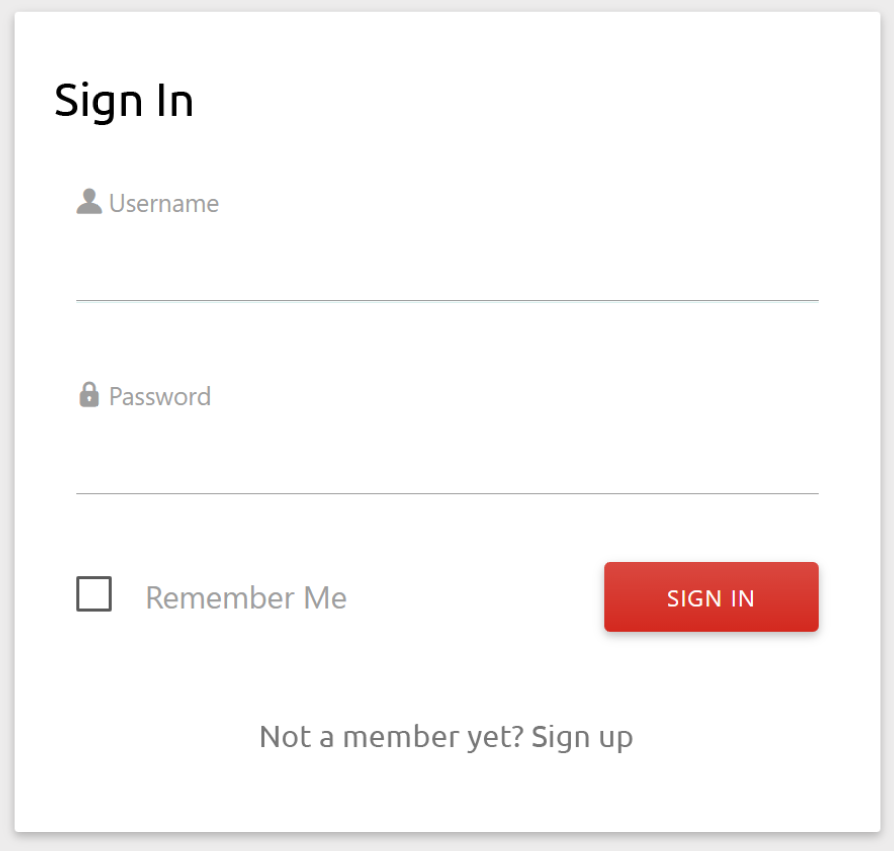
\includegraphics[width=0.75\textwidth]{signin}
\end{figure}

\subsection{Registration}
All users must register in order to use ClinicFlow. Registration is simple, and requires only a username and password.
\medbreak

If you already have an account, please refer to Login (4.1)
\medbreak

To Sign Up:
\medbreak
1. Enter a desired username into the Username field (must be unique)
\medbreak
2. Enter a password into the password field (must adhere to security requirements)
\medbreak
- Between 8 and 20 characters
\medbreak
- Contain at least 1 number and 1 symbol
\medbreak
3. Click the "I am not a robot" checkbox.
\medbreak
4. Click "Sign up"

\begin{figure}[h]
\caption{Sign up page}
\centering
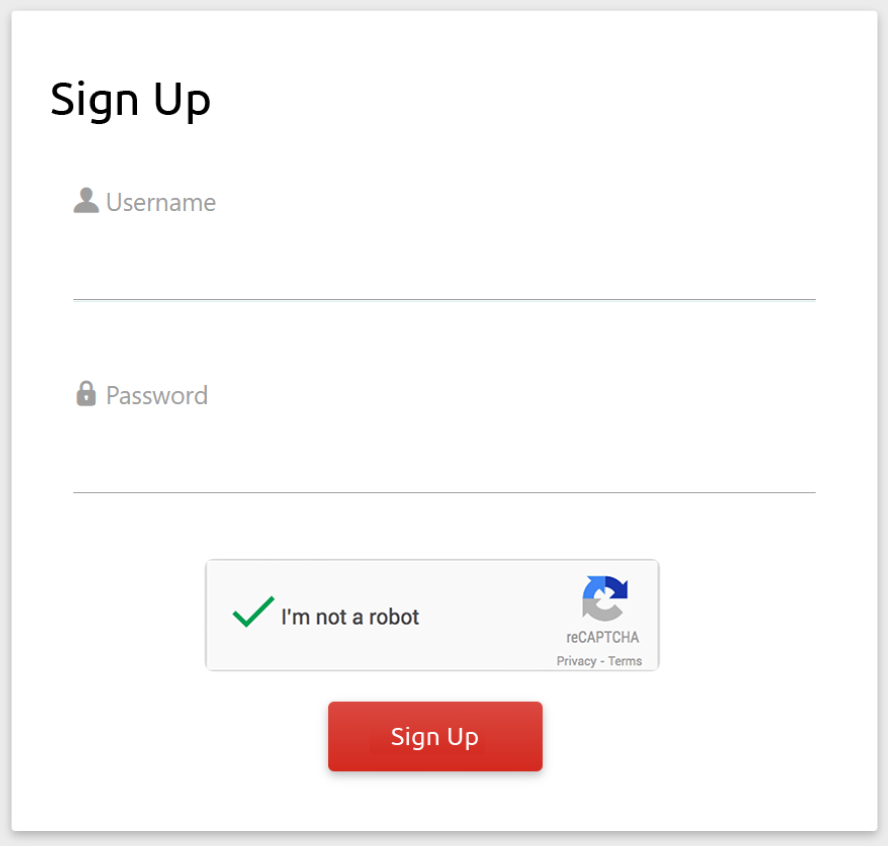
\includegraphics[width=0.8\textwidth]{signup}
\end{figure}

\section{Dashboard}
\subsection{Clinic}
Upon logging in, the user will be presented the clinic selection screen. From here they can either select the clinic to use, or create a new clinic.
\medbreak

If no clinic is associated with this account, one must be created (See 5.1.1)

\subsubsection{Create Clinic}
To use this application, a clinic must be created it's constraints set up.
\medbreak
To create clinic, one must be on the "Choose Clinic screen" (See figure 4)
\medbreak

To create a clinic:
\medbreak
1. Click the "Create Clinic" button
\medbreak
2. Enter the clinic name (must be unique)
\medbreak
3. Enter clinic constraints
\medbreak
3.1 Services: list the services available to the patients
\medbreak
3.2 Providers: Set type and number of staff, including breaks and administered services
\medbreak
4. Click "Create New Clinic"
\medbreak

\begin{figure}[h]
\caption{Creating a new clinics}
\centering
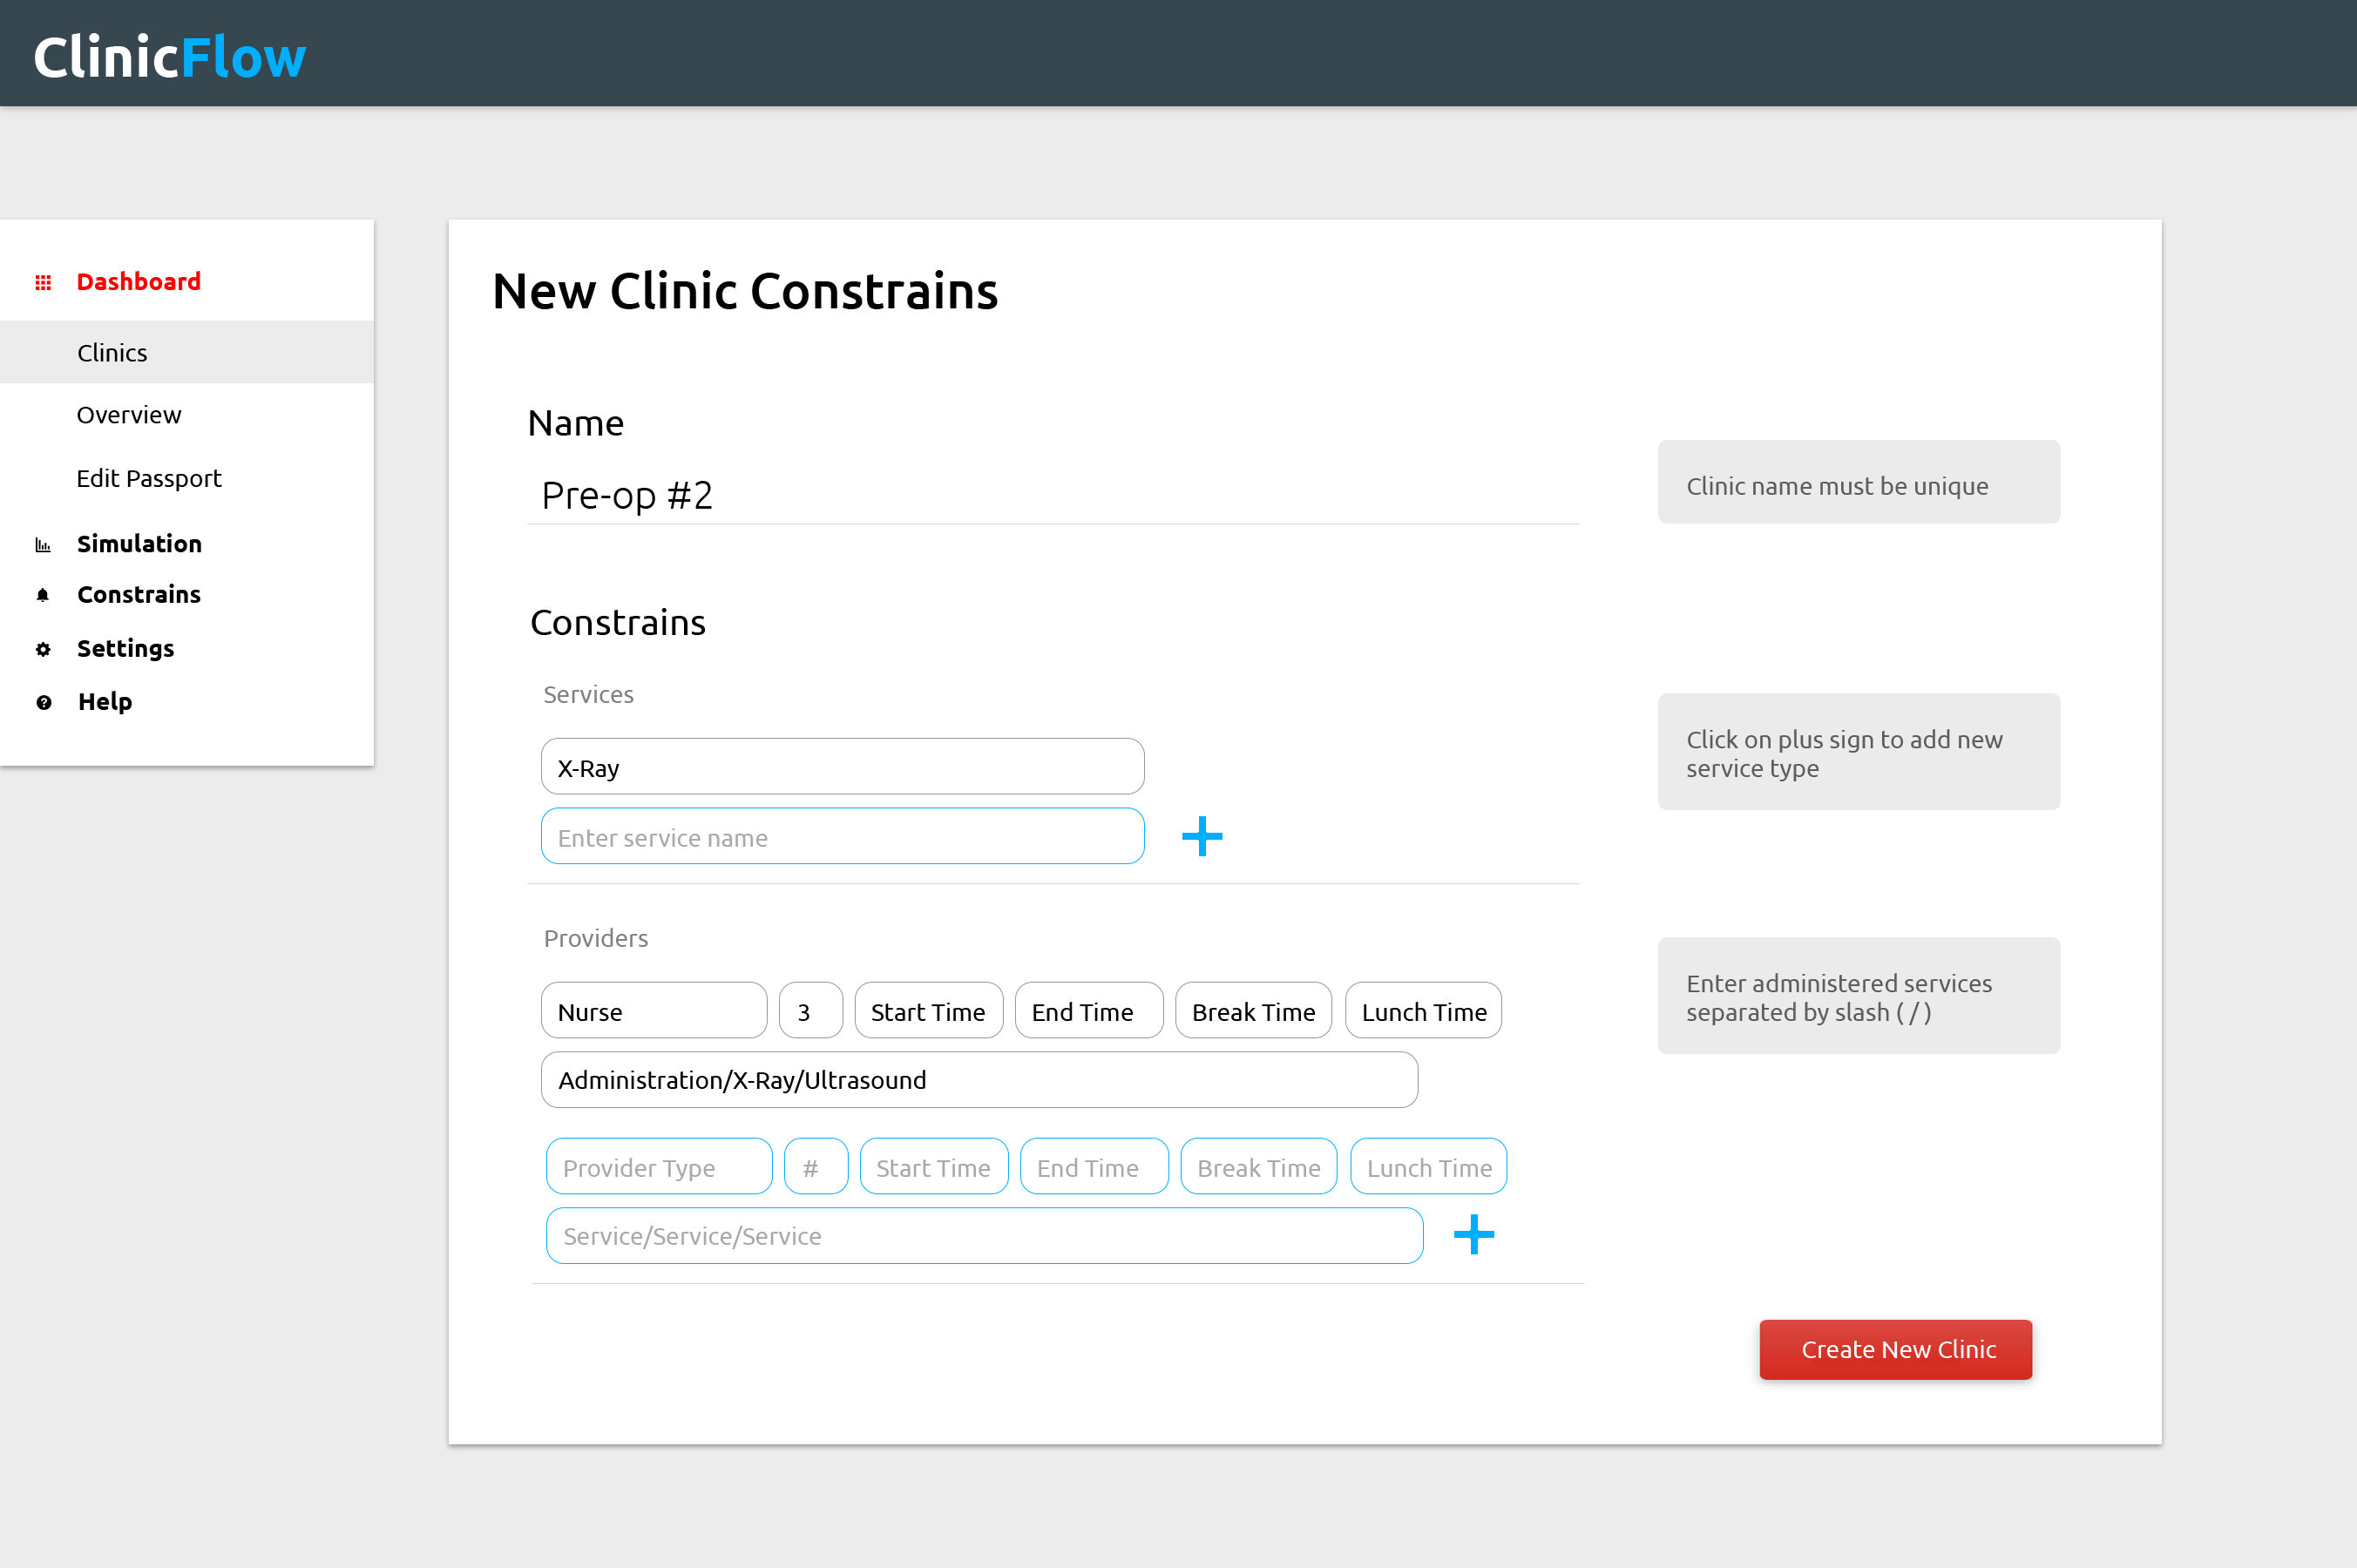
\includegraphics[width=\textwidth]{newclinic}
\end{figure}

\subsubsection{Select Clinic}
To select a clinic, click on one of the clinics in the list. (See figure X3)
\medbreak

Note: A clinic must be created in order to select a clinic (See 5.1.1)

\begin{figure}[h]
\caption{Select from created clinics}
\centering
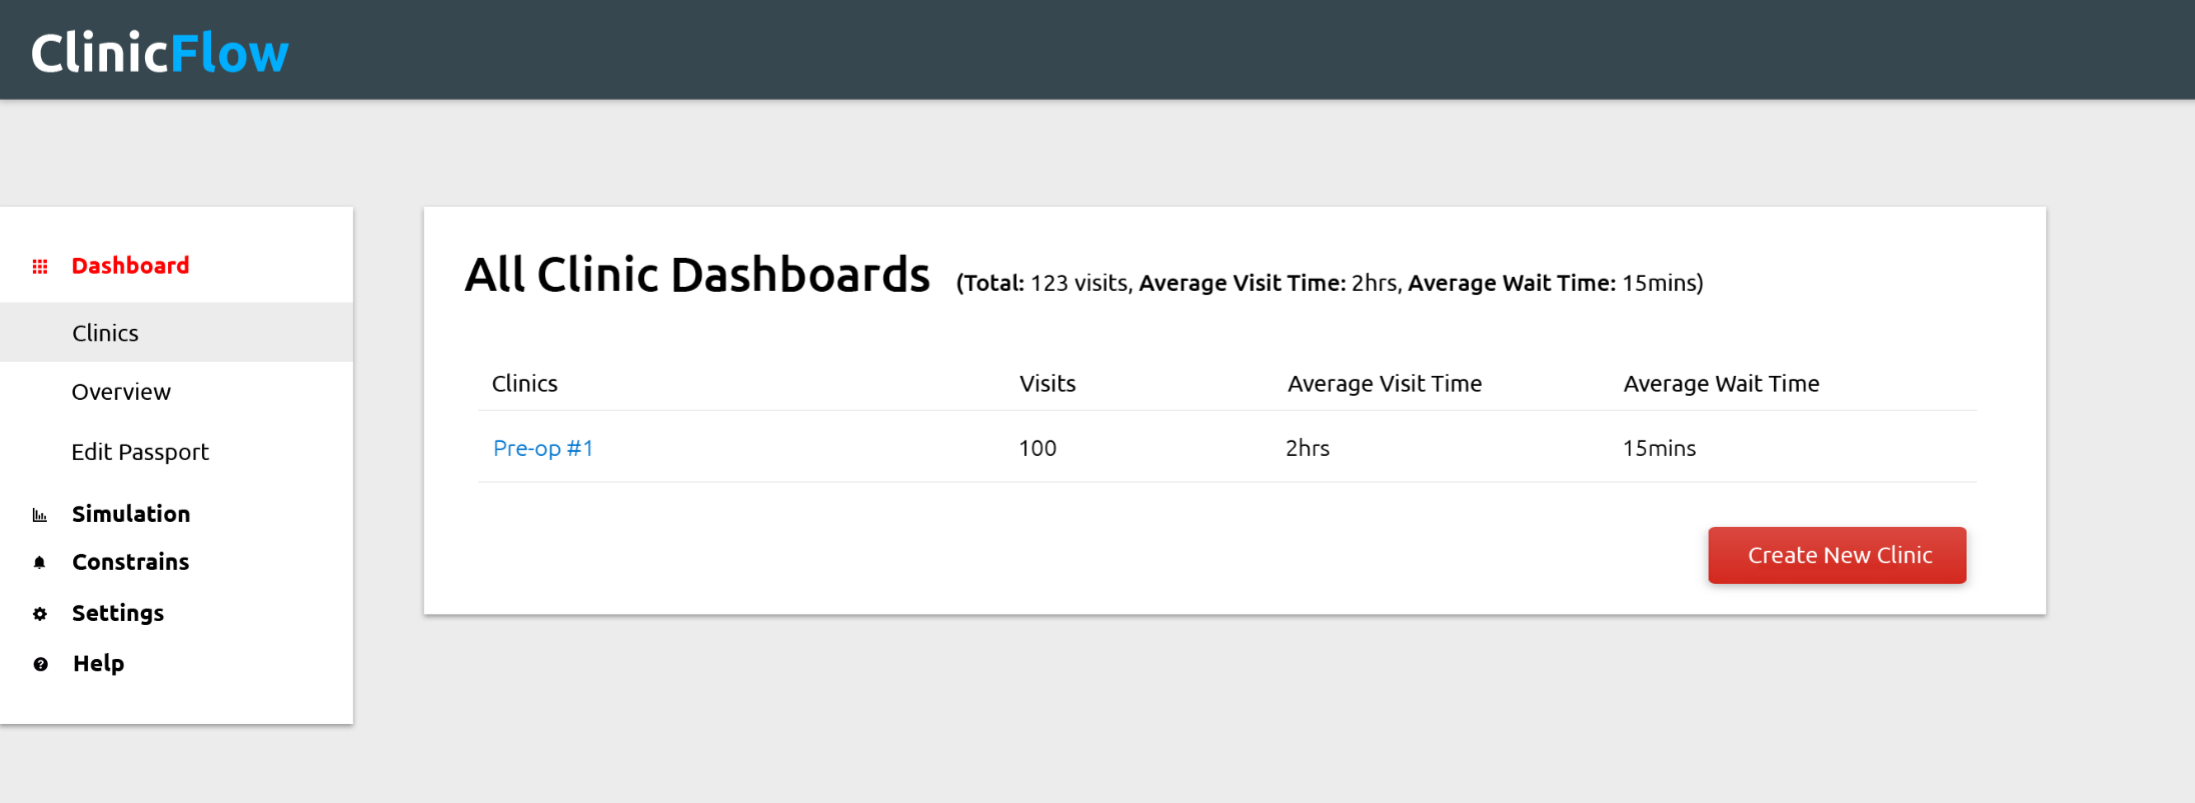
\includegraphics[width=\textwidth]{selectclinic}
\end{figure}

\subsection{Overview}
This screen will show statistic about the current status of the clinic based on actual passport data.
\medbreak

Note: clinic passport data must be set up in order to use this screen (See 5.3)

\subsubsection{Select Date Range}
The selects the time range for which statistics will be calculated.
\medbreak

In order to change:
\medbreak
1. Click on the arrow beside the date at the top
\medbreak
2. Select the FROM date on the left
\medbreak
3. Select the TO date on the right
\medbreak
4. Click apply to filter the passport data to within that range
\pagebreak

\begin{figure}[h!]
\caption{overview of clinic}
\centering
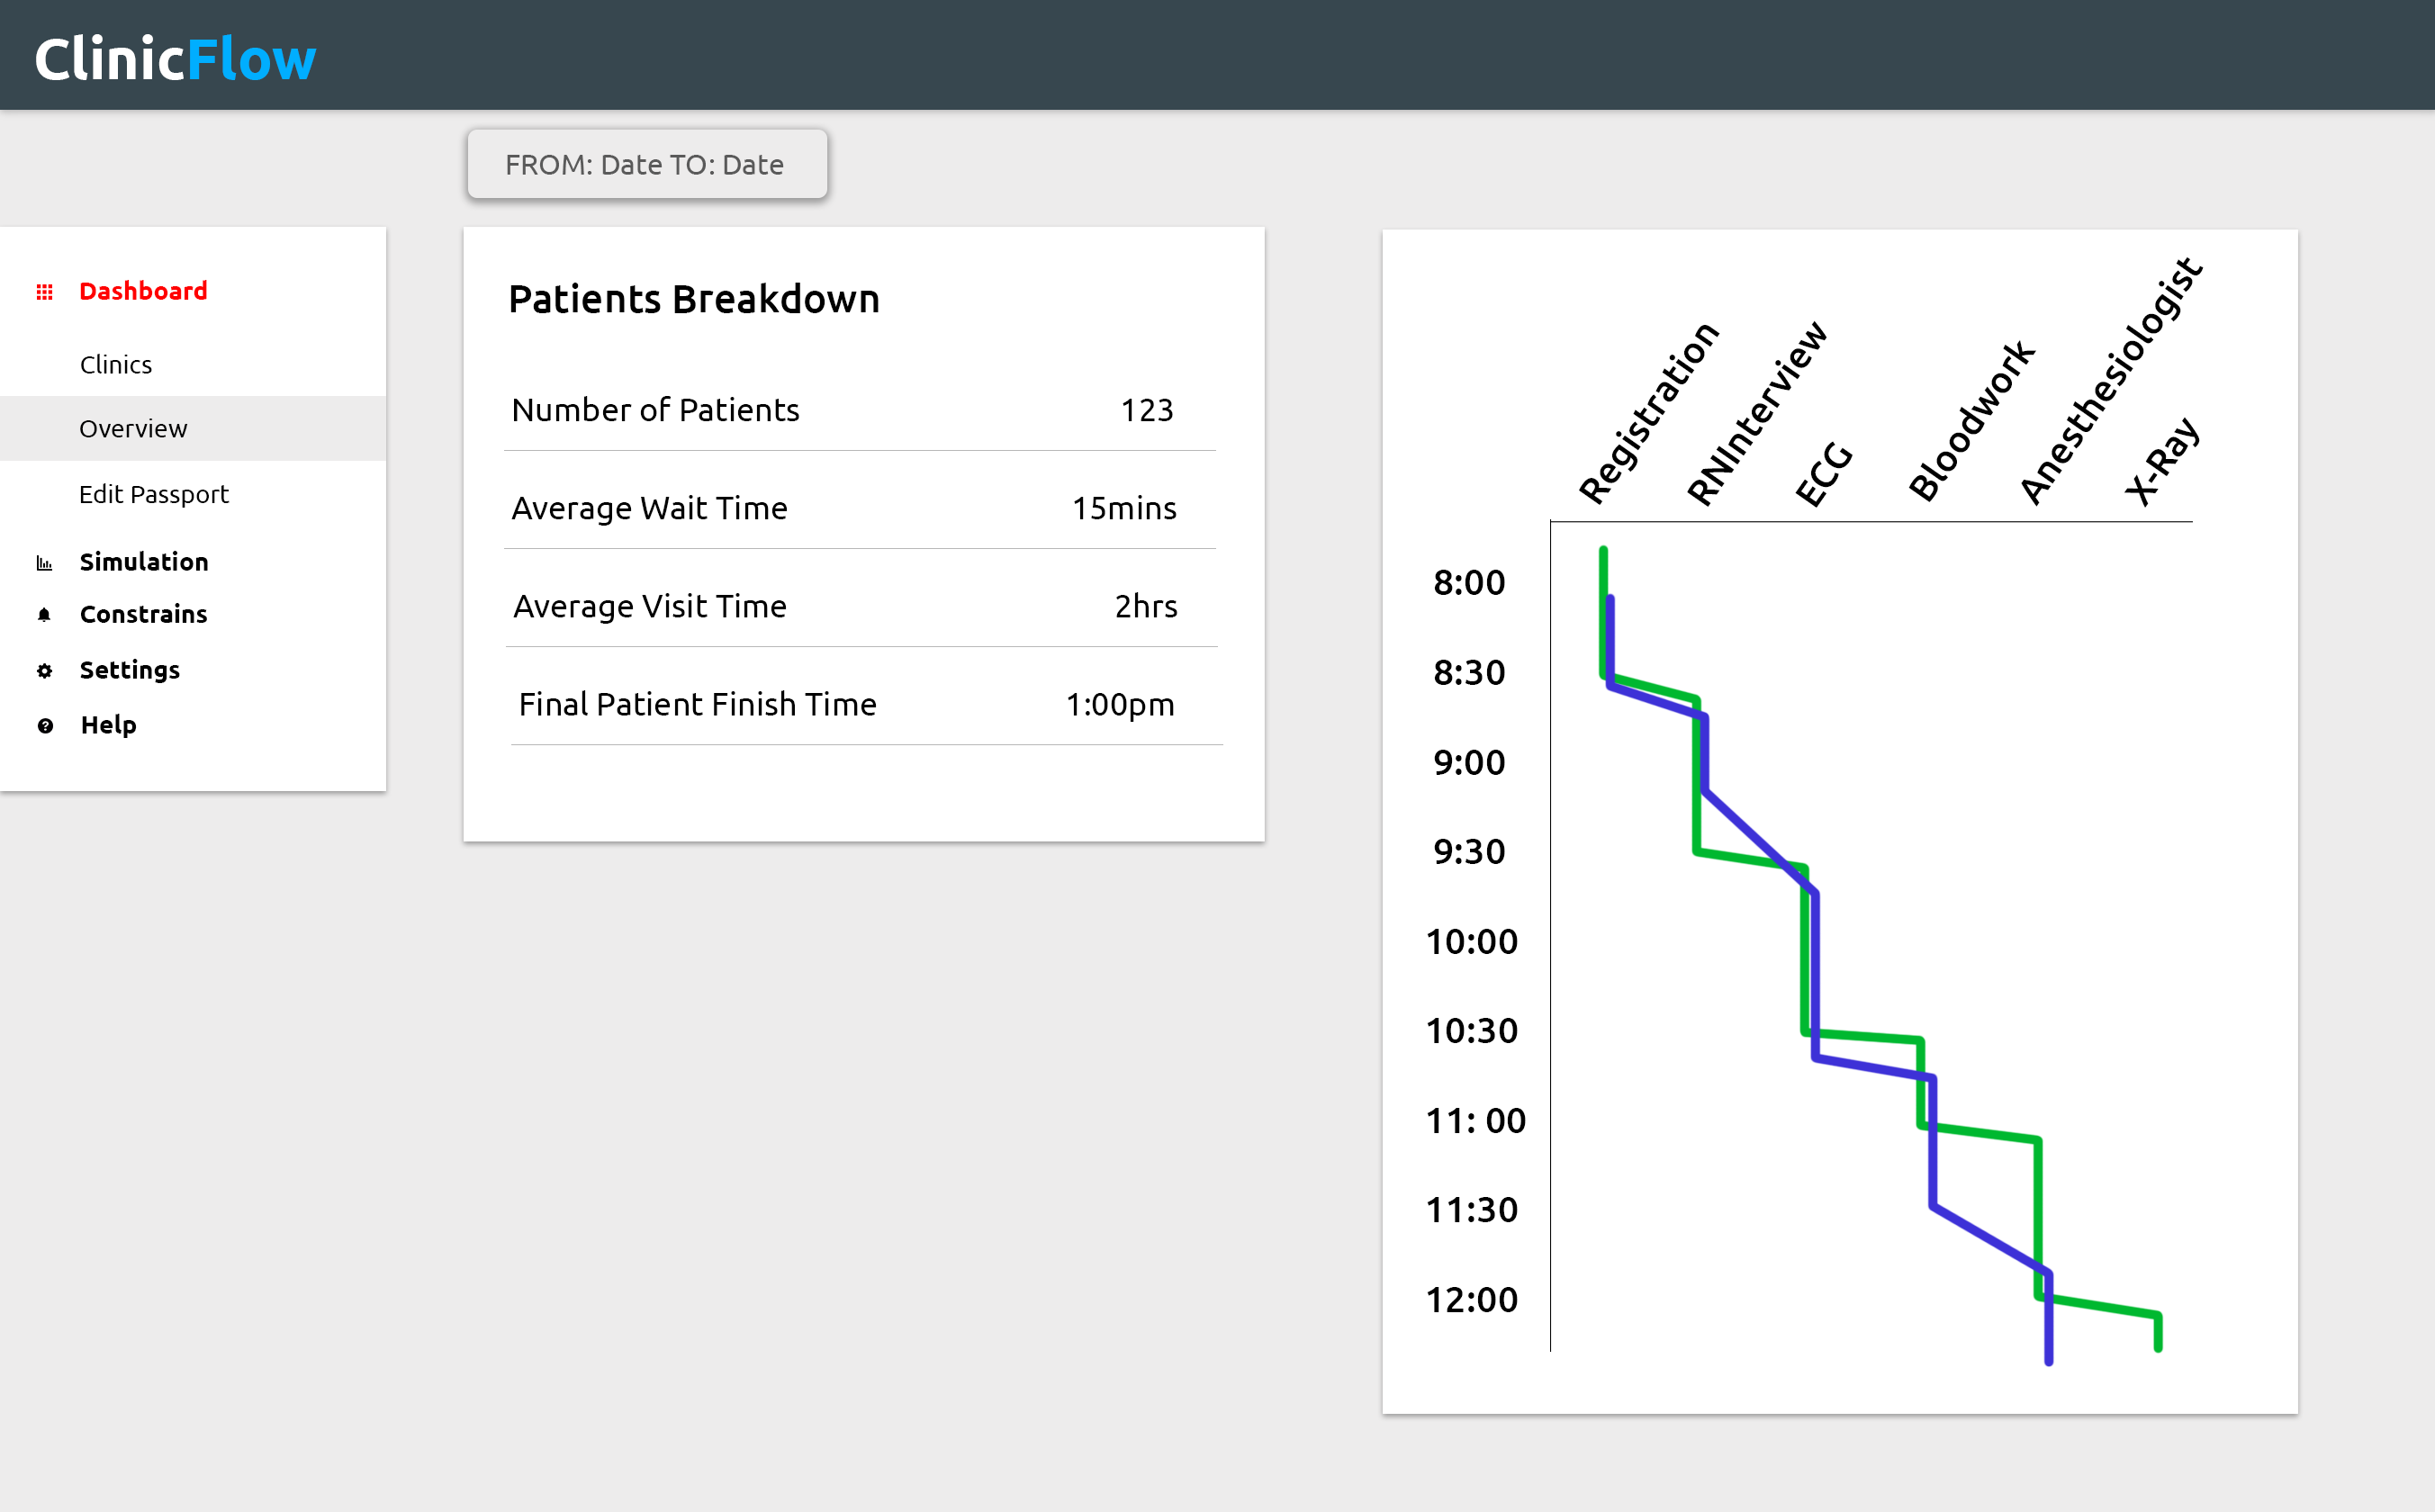
\includegraphics[width=\textwidth]{overview}
\end{figure}

\subsection{Edit Passport}
This section allow the user to edit past actual data. This data is used to provide summary statistics of the clinic environment, as well as help build a model of the clinic for simulation purposes.
\medbreak

Note: In order to edit passport, the clinic must have a set of constraints associated with it (See 5.5)
\medbreak

To add a patient:
\medbreak
1. Click the "Add patient" button
\medbreak
2. Enter the patient information, including name/id, scheduled arrival time, and required procedures
\medbreak
3. Click "Apply"
\medbreak

To remove a patient:
\medbreak
1. Click the "X" button beside the patient name in the list
\medbreak
2. Click "Apply"

\subsection{Simulate}
This section of the application allows the user to simulate a model clinic environment.
\medbreak

If no schedule/rule set has been created, the user must create one first (See 5.4.2)

\subsubsection{Simulation Selection}
This screen shows a list of stored simulation models.
\medbreak

To select a simulation, click on the name of simulation.

\subsubsection{Create Model}
This function allow the user to create a new simulation model. This is required in order to run simulations.
\medbreak

\begin{figure}[h!]
\caption{Creating simulation}
\centering
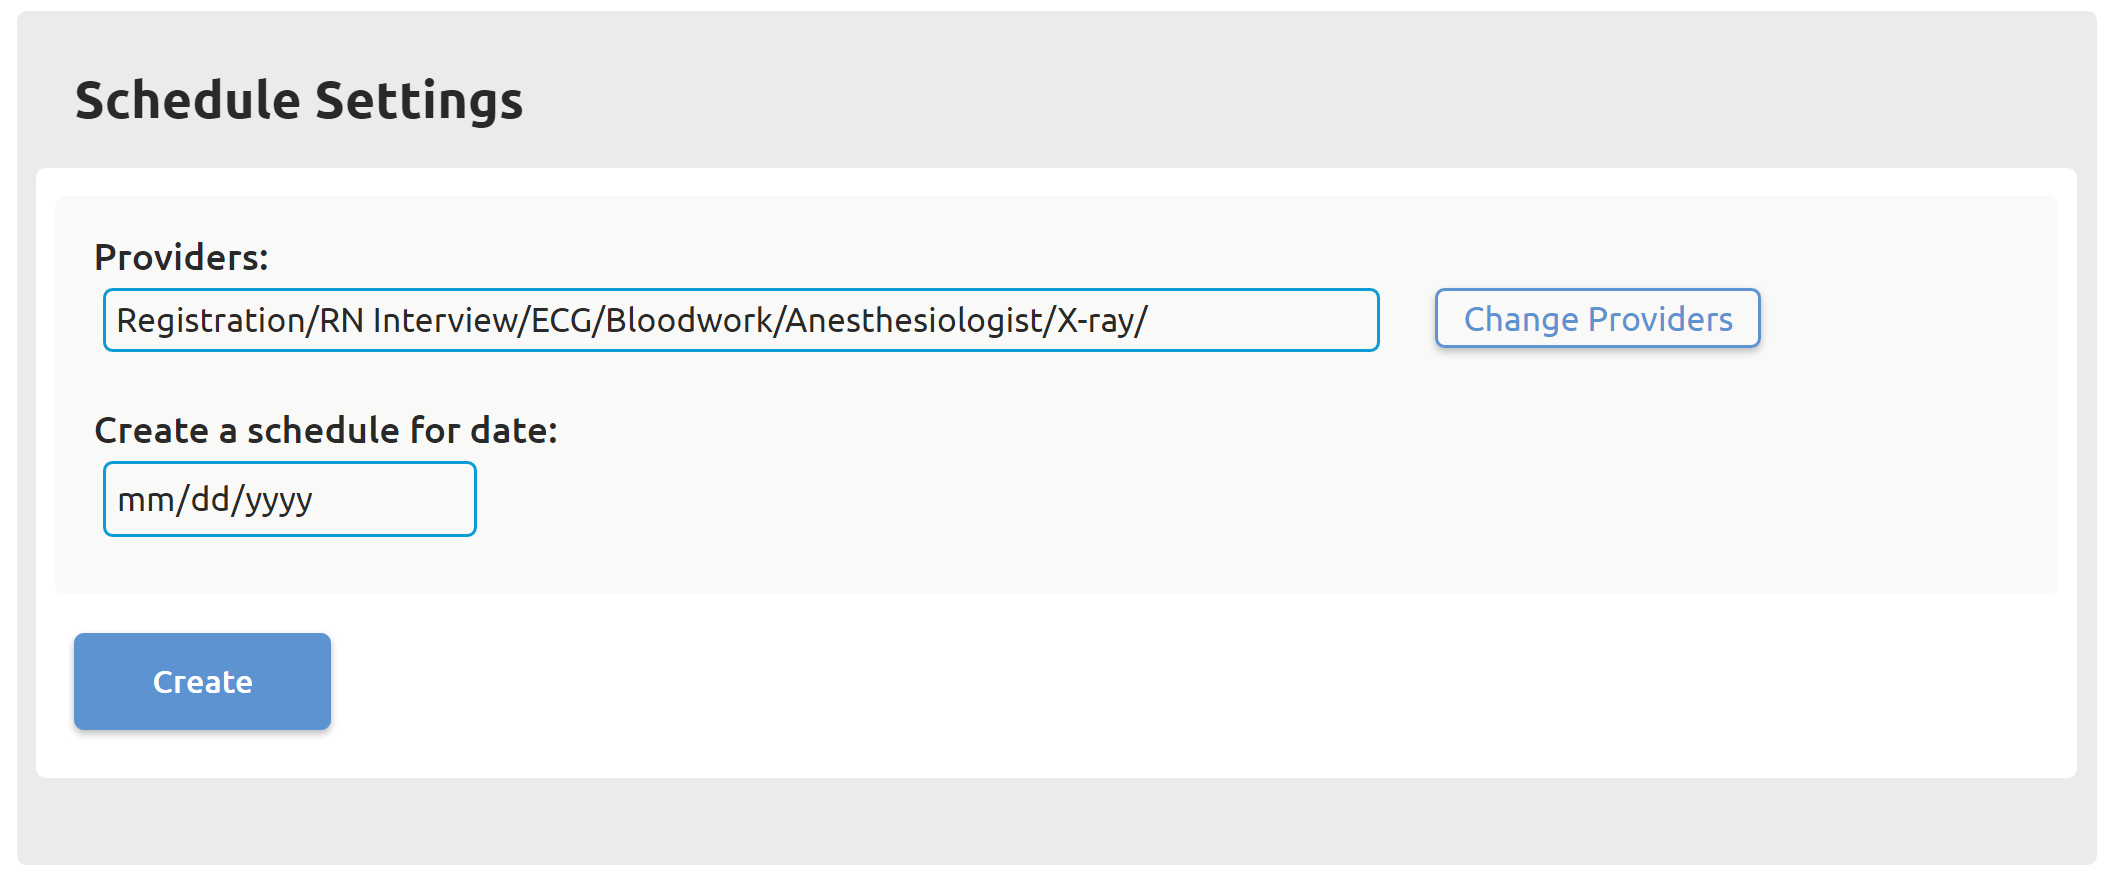
\includegraphics[width=\textwidth]{simsetting}
\end{figure}

To create a simulation model:
\medbreak
1. Click "Create Model"
\medbreak
2. Click "Use constraint info" (skip to 5.) or Fill in details (steps 3-4)
\medbreak
3. Enter patients to simulate
\medbreak
3.1 Click "Add patient"
\medbreak
3.2 Enter name, arrival time, and required procedures
\medbreak
4. Enter constraints to adhere to
\medbreak
4.1 Enter providers, staff, and prerequisites
\medbreak
5. Click "Create"

\begin{figure}[h!]
\caption{Add patients to simulation}
\centering
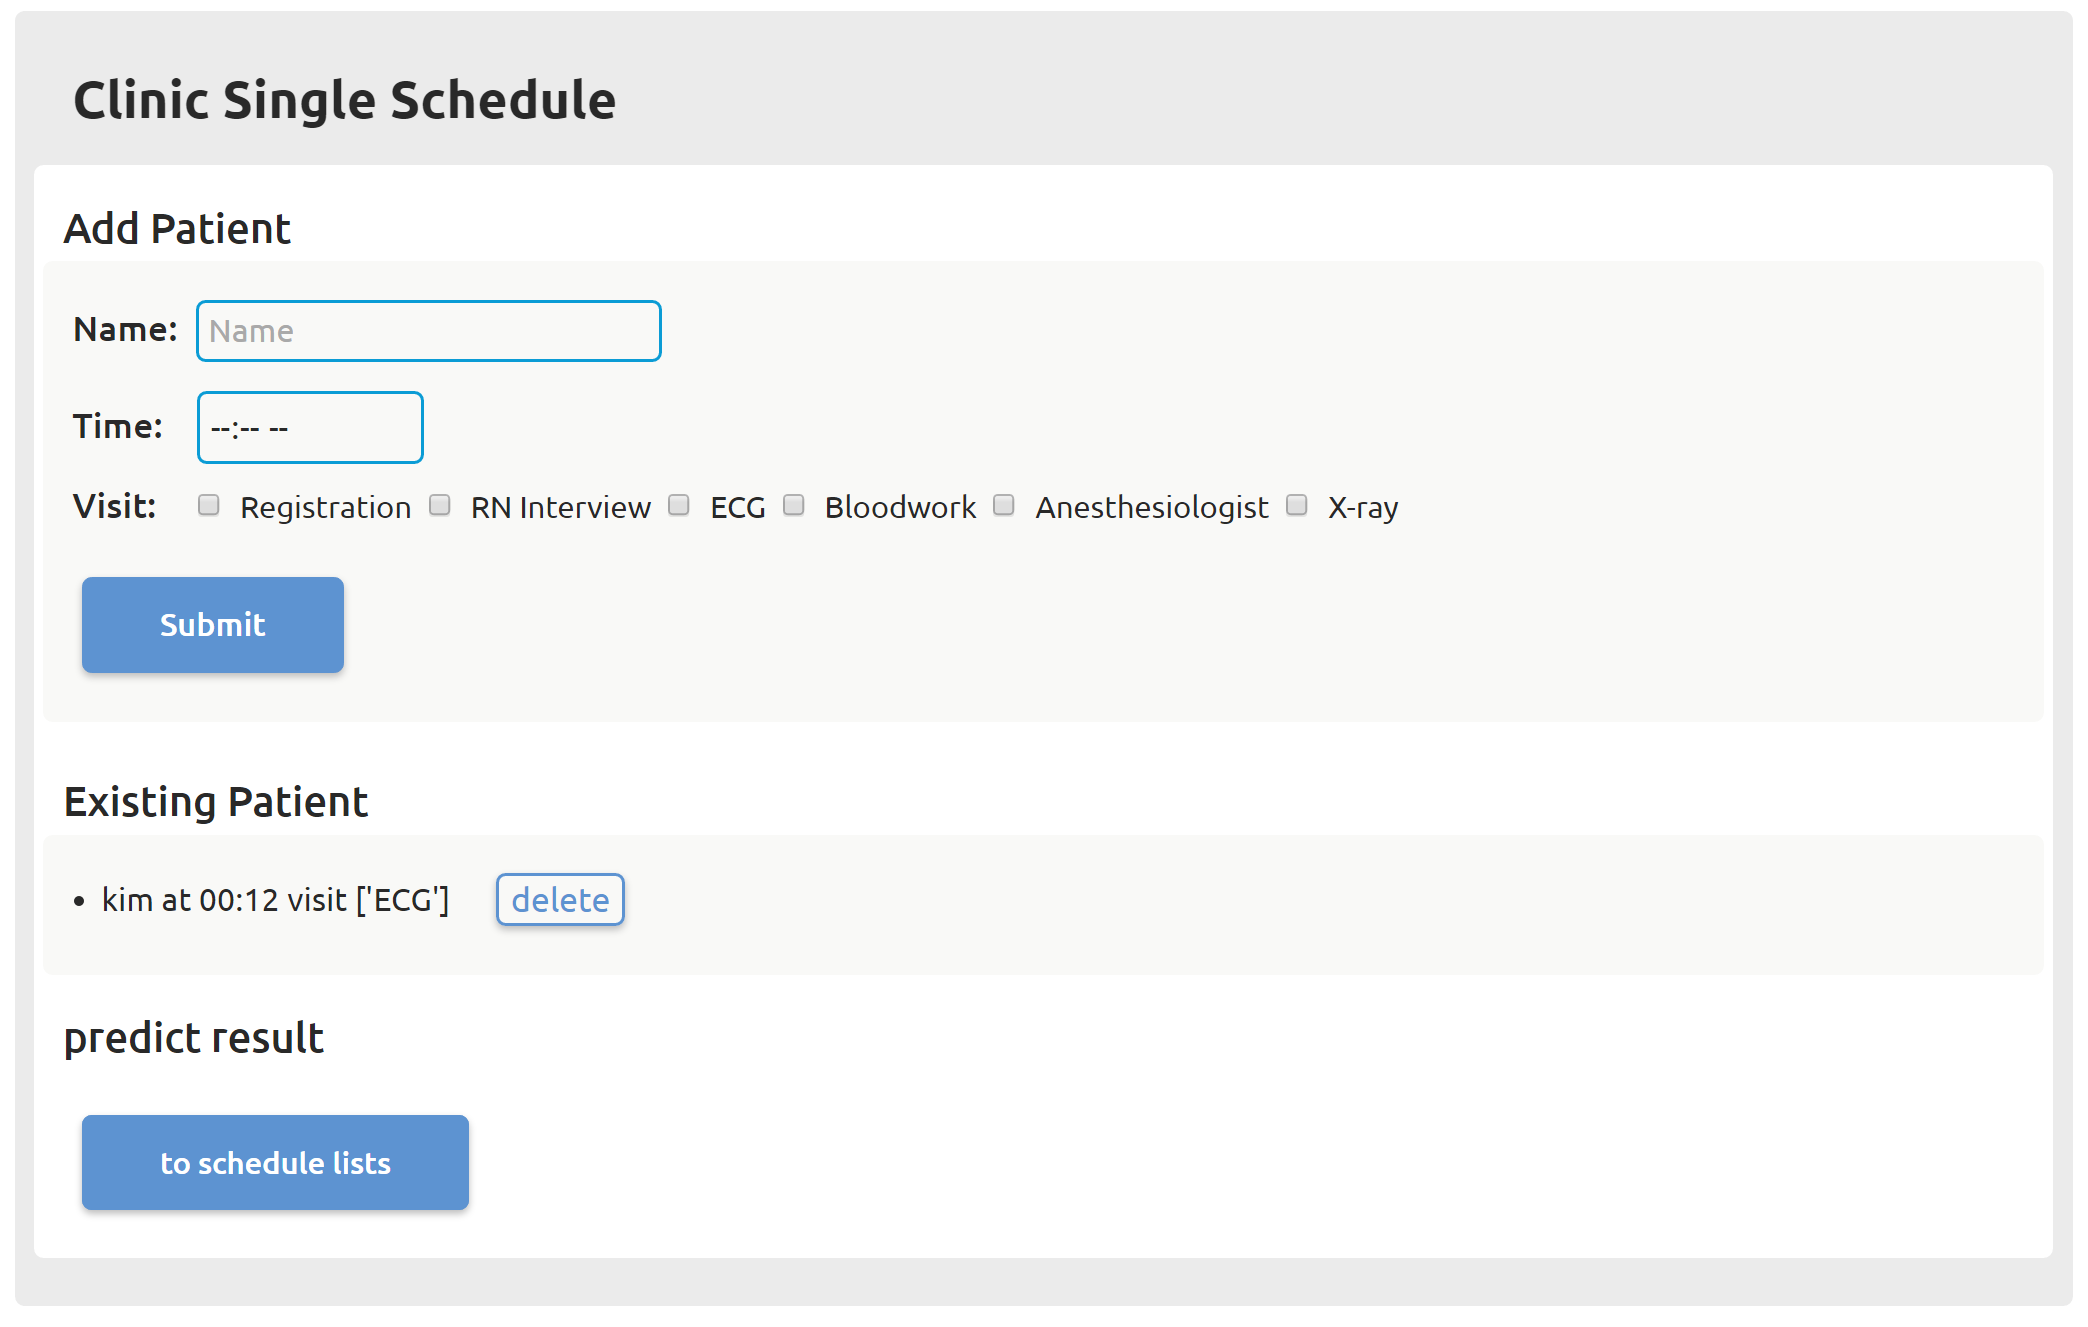
\includegraphics[width=\textwidth]{sim}
\end{figure}

\subsubsection{Results}
This screen shows statistics from the last simulation. If no simulation has been performed, only the simulation selection screen will be visible.
\medbreak

In order to simulate a model, click on the "Simulate" button beside the model in the list.
\medbreak

The results screen shows statistics such as mean procedure time, waiting time, total clinic operation time.

\subsection{Constraints}
This section allows the user to change the constraints for the current clinic.
\medbreak

All 3 sections must have their properties set in order to use the passport feature, as well as to use constraint info in a simulation model.

\subsubsection{Change Providers / prerequisites / staff}
This section allow the user to set the list of providers available in the clinic.
\medbreak

In order to add a provider:
\medbreak
1. Click the "+" button under "Providers" to add an additional provider.
\medbreak
2. Enter the name of the provider in the new text box
\medbreak
3. Click Apply to save the list of providers
\medbreak

In order to set the prerequisites:
\medbreak
1. Click the "+" button under "Prerequisites" to add a prerequisite
\medbreak
2. Enter the before procedure
\medbreak
3. Enter the after procedure
\medbreak
4. Click "Apply' to save the list of prerequisites
\medbreak

In order to set the staff:
\medbreak
1. Click the "+" button under "Staff" to add a staff member
\medbreak
2. Enter their name
\medbreak
3. Enter the procedures they can provide
\medbreak
4. Enter their start, end, and break times.
\medbreak
5. Click "Apply" to save the list of staff

\subsection{Settings}
This section allows the user to change setting related to their account

\subsubsection{Change Password}
The user can change the password for their account:
\medbreak
1. Click on "Change Password"
\medbreak
2. Enter current password
\medbreak
3. Enter current password again
\medbreak
4. Enter new password
\medbreak
5. Click "Apply"

\subsubsection{Change Clinic Name}
The user can change the name of any clinic associated with their account
To do this:
\medbreak
1. Click "Change clinic name"
\medbreak
2. Select clinic whose name to change
\medbreak
3. Enter new name for clinic
\medbreak
4. Click "Apply"

\section{Troubleshooting}
\subsection{FAQ}
This section provides information on commonly asked questions regarding the operation of product.
\medbreak

1. Why do I not see a list of clinics?
\medbreak
1- You must be signed in, and have at least 1 clinic create in order to see the list of clinics. See 4.1, 5.1.1.
\medbreak

2. Why do I not see a passport?
\medbreak
2- You must enter the clinic constraints and patient data in order to see the passport and statistics. See 5.5, 5.3

\subsection{Contact Us}
If you have any further questions contact us at:
\medbreak
- vasiliem@mmcaster.ca
\medbreak
- knopfk@mcmaster.ca
\medbreak
- yum27@mcmaster.ca
\medbreak
- huw7@mcmaster.ca
\medbreak
- li544@mcmaster.ca

\section{Definitions}
Account: An entity identified by username and password credentials. Contains clinics.
\medbreak\medbreak
Clinic: An entity consisting of a passport and constraints.
\medbreak\medbreak
Passport: A spreadsheet of past clinic data, including patient arrival time, procedure duration, and departure time.
\medbreak\medbreak
Constraints: Rules regarding clinic behavior, used in simulation

\end{document}
